%%
%% Class homework & solution template for latex
%% Alex Ihler
%%
\documentclass[twoside,11pt]{article}
\usepackage{amsmath,amsfonts,amssymb,amsthm}
\usepackage{graphicx,color}
\usepackage{verbatim,url}
\usepackage{listings}
\usepackage{upquote}
\usepackage[T1]{fontenc}
%\usepackage{lmodern}
\usepackage[scaled]{beramono}
%\usepackage{textcomp}

% Directories for other source files and images
\newcommand{\bibtexdir}{../bib}
\newcommand{\figdir}{fig}

\newcommand{\E}{\mathrm{E}}
\newcommand{\Var}{\mathrm{Var}}
\newcommand{\N}{\mathcal{N}}
\newcommand{\matlab}{{\sc Matlab}\ }

\setlength{\textheight}{9in} \setlength{\textwidth}{6.5in}
\setlength{\oddsidemargin}{-.25in}  % Centers text.
\setlength{\evensidemargin}{-.25in} %
\setlength{\topmargin}{0in} %
\setlength{\headheight}{0in} %
\setlength{\headsep}{0in} %

\renewcommand{\labelenumi}{(\alph{enumi})}
\renewcommand{\labelenumii}{(\arabic{enumii})}

\theoremstyle{definition}
\newtheorem{MatEx}{M{\scriptsize{ATLAB}} Usage Example}

\definecolor{comments}{rgb}{0,.5,0}
\definecolor{backgnd}{rgb}{.95,.95,.95}
\definecolor{string}{rgb}{.2,.2,.2}
\lstset{language=Matlab}
\lstset{basicstyle=\small\ttfamily,
        mathescape=true,
        emptylines=1, showlines=true,
        backgroundcolor=\color{backgnd},
        commentstyle=\color{comments}\ttfamily, %\rmfamily,
        stringstyle=\color{string}\ttfamily,
        keywordstyle=\ttfamily, %\normalfont,
        showstringspaces=false}
\newcommand{\matp}{\mathbf{\gg}}




\begin{document}

\centerline{\Large Homework 5}
\centerline{Zachary DeStefano, 15247592}
\centerline{CS 273A: Winter 2015}
\centerline{\bf Due: March 10, 2015}

\section*{Problem 1}

\subsection*{Part a}

The data does not look very clustered. Here is the plot of the raw data:

\begin{figure}[h]
\centering
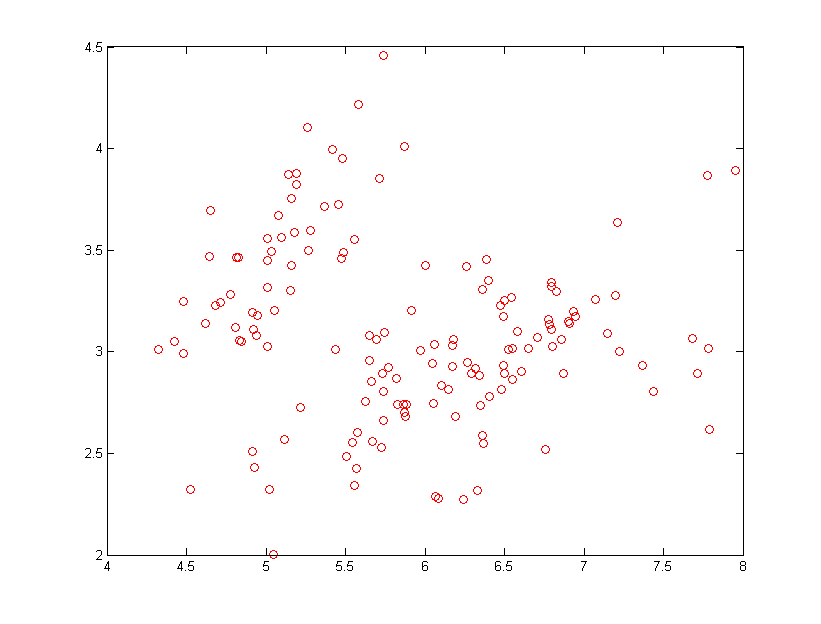
\includegraphics[width=6 in]{prob1PartA.png}
\caption{Raw Iris Data}
\end{figure}

\newpage

\subsection*{Part b}

I tried a few different initializations. I tried the 3 different ones available in the kmeans function as well as my own initialization points. For $k=5$, I arranged 5 points in an X-shape in the $x_1,x_2$ space. For $k=20$, I did two different initial arrangements: a $4x5$ grid and a $5x4$ grid in the $x_1,x_2$ space. For $k=5$ the lowest score came from my initialization. For $k=20$ the lowest score also came from my initialization, specifically the $5x4$ initialization, although the $4x5$ grid had nearly the same score. \\
\\
Here is the best 5-means clustering I was able to achieve
\begin{figure}[h]
\centering
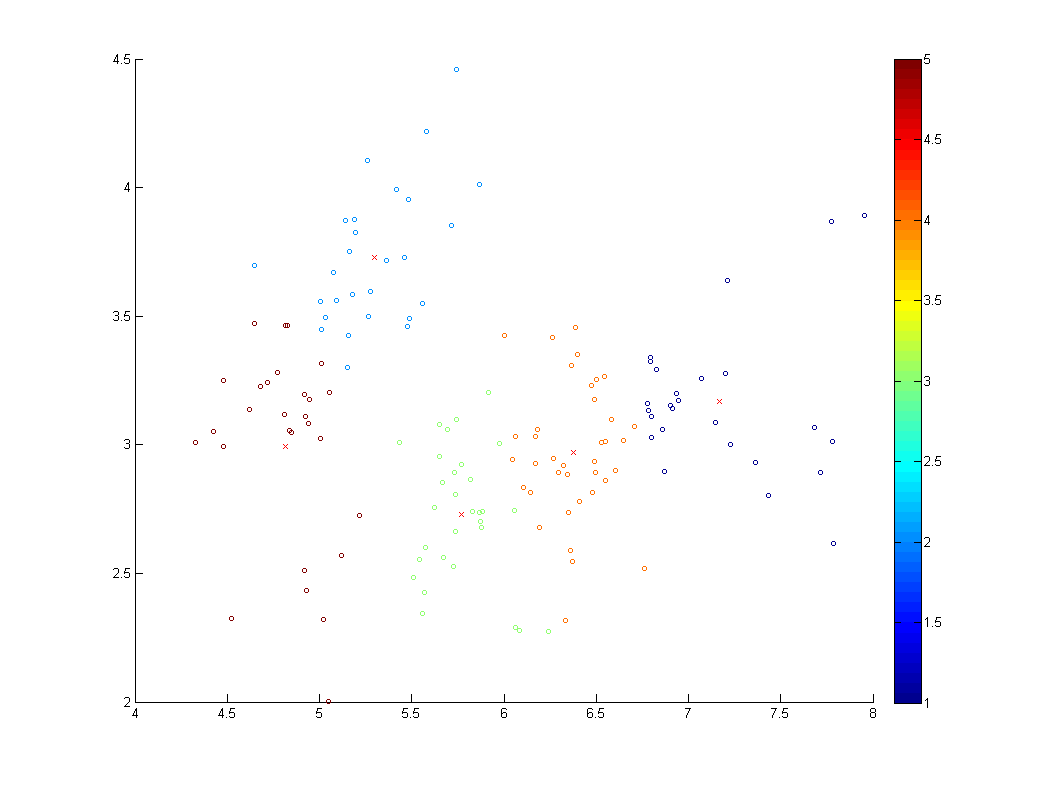
\includegraphics[width=6 in]{prob1PartB_1.png}
\caption{$k=5$ clustering with x marks for cluster centers}
\end{figure}

\newpage

Here is the best 20-means clustering I was able to achieve.
\begin{figure}[h]
\centering
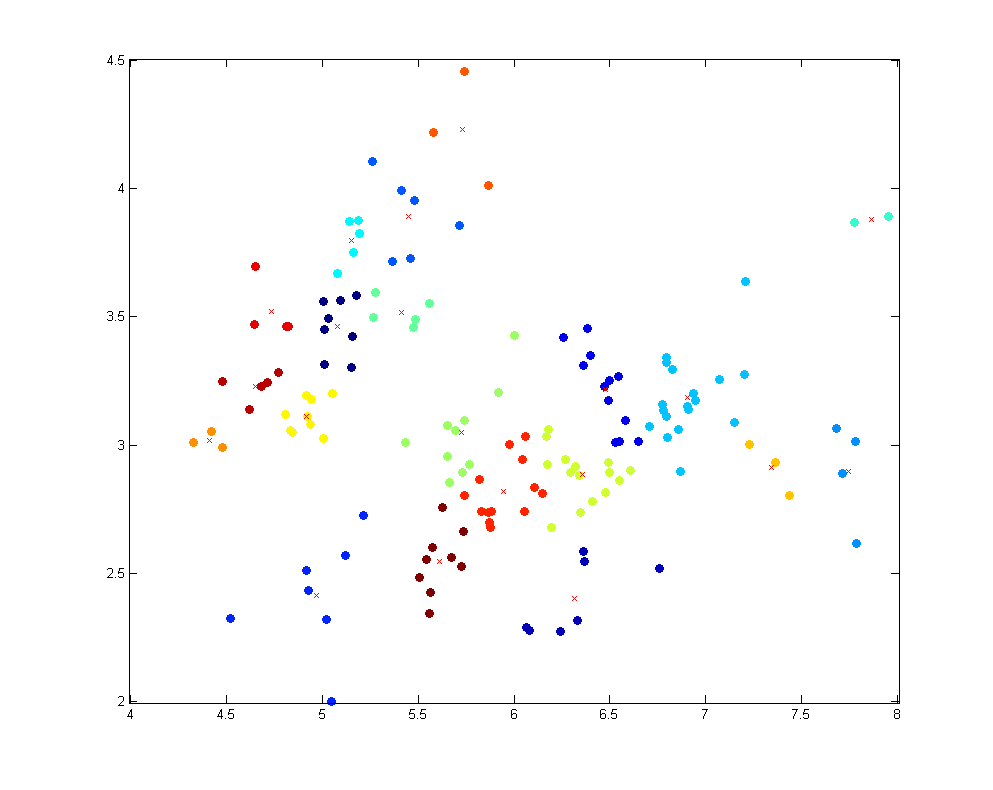
\includegraphics[width=6 in]{prob1PartB_2.png}
\caption{$k=20$ clustering with x marks for cluster centers}
\end{figure}

\newpage

Here is the code for Part A and B.
\lstinputlisting[firstline=1, lastline=93]{prob1.m}

\newpage

\subsection*{Part c}

Here are the plots of agglomerative clustering with 5 clusters.  
\begin{figure}[h]
\centering
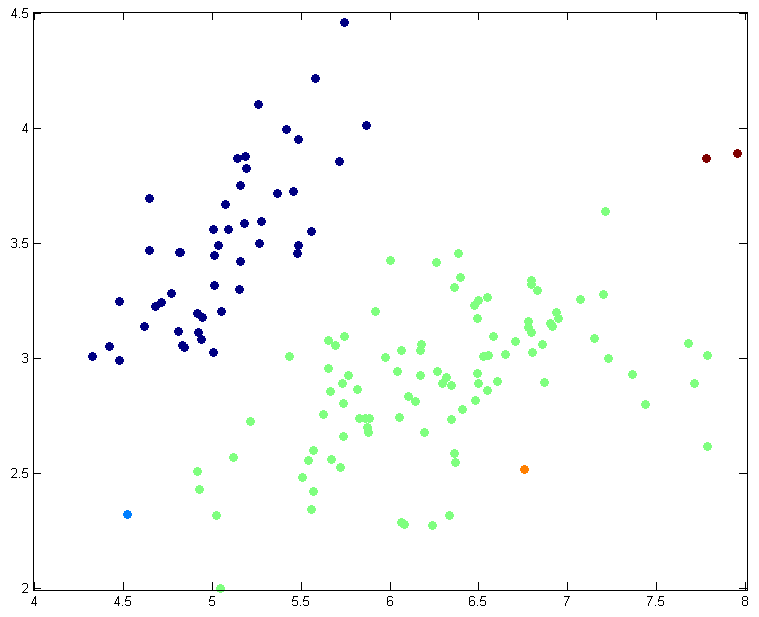
\includegraphics[width=6 in]{prob1PartC_1.png}
\caption{Agglomerative clustering with 5 clusters, single linkage}
\end{figure}

\newpage

\begin{figure}[h]
\centering
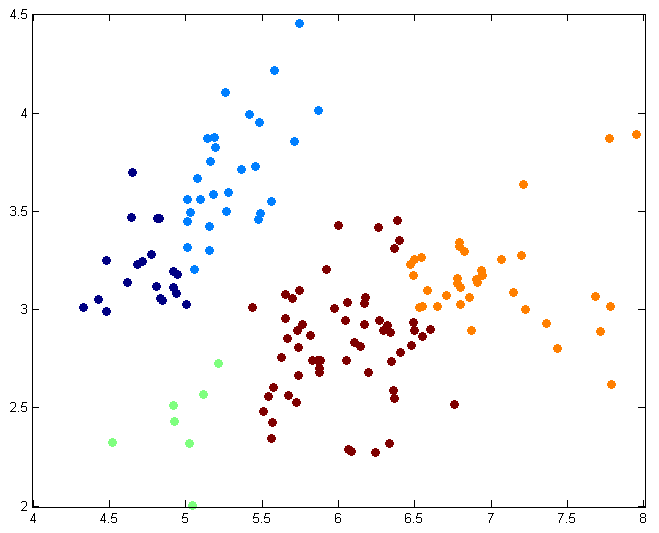
\includegraphics[width=6 in]{prob1PartC_2.png}
\caption{Agglomerative clustering with 5 clusters, complete linkage}
\end{figure}

\newpage

Here are the plots of agglomerative clustering with 20 clusters.  
\begin{figure}[h]
\centering
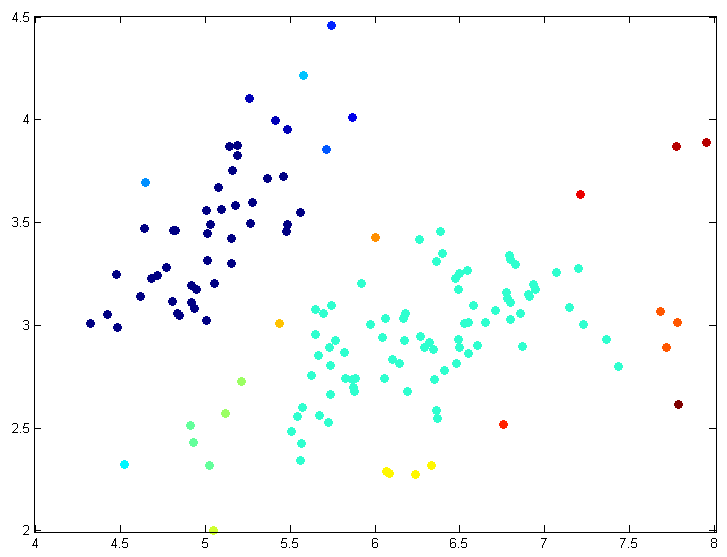
\includegraphics[width=6 in]{prob1PartC_3.png}
\caption{Agglomerative clustering with 20 clusters, single linkage}
\end{figure}

\newpage

\begin{figure}[h]
\centering
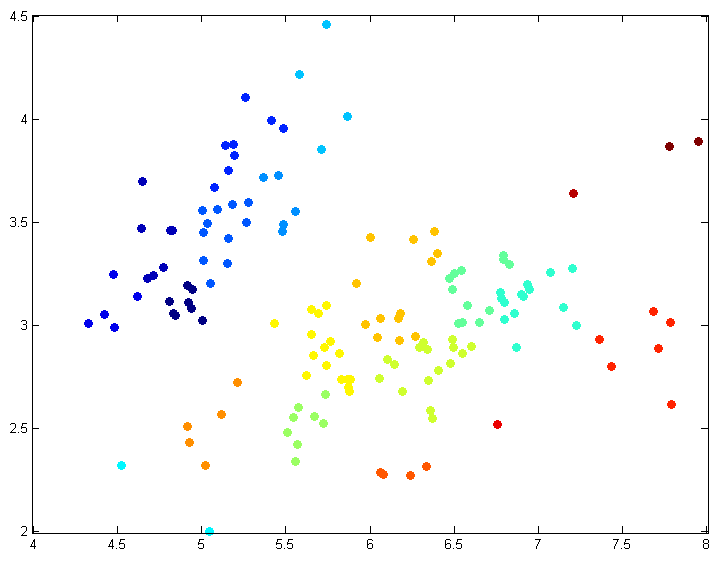
\includegraphics[width=6 in]{prob1PartC_4.png}
\caption{Agglomerative clustering with 20 clusters, complete linkage}
\end{figure}

\newpage 
As can be observed, single linkage tries to group the points into as few clusters as possible whereas complete linkage spreads out the clustering. The results for complete linkage look quite similar to k-Means. \\
\\
Here is the code for Part C\\
\lstinputlisting[firstline=95, lastline=103]{prob1.m}

\newpage

\subsection*{Part d}

Here is the plot of 5 clusters found using EM
\begin{figure}[h]
\centering
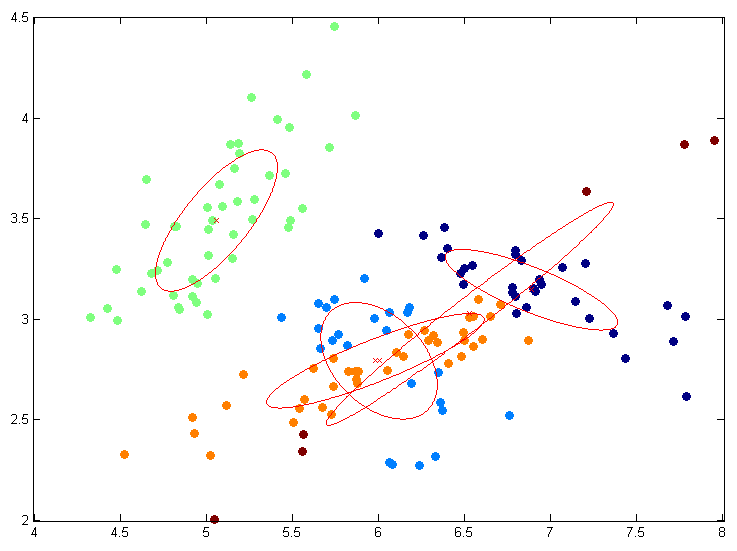
\includegraphics[width=6 in]{prob1PartD_1.png}
\caption{EM run to figure out 5 clusters}
\end{figure}
\newpage
Here is the plot of 20 clusters found using EM
\begin{figure}[h]
\centering
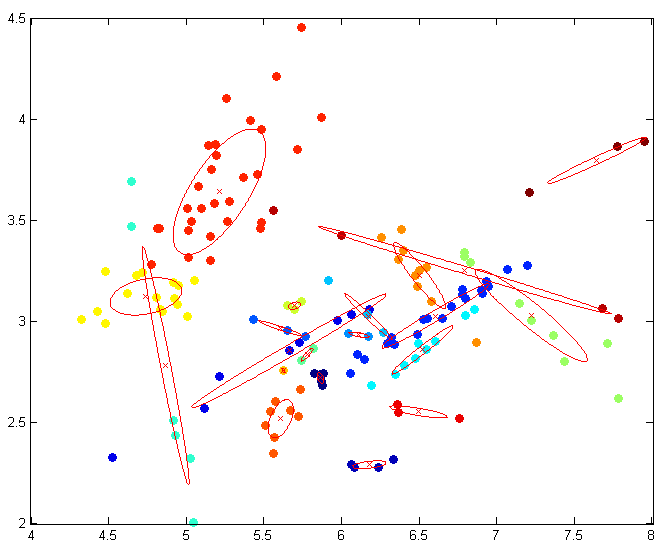
\includegraphics[width=6 in]{prob1PartD_2.png}
\caption{EM run to figure out 20 clusters}
\end{figure}

\newpage

I used the same initializations as k-means, including the points I constructed. The score I used was the log likelihood. With this score, the higher the better. The best log likelihood I achieved occurred when I specified points. This is similar to what happened when I did k-Means. \\
\\
Overall, k-Means clustering seems to be the most reasonable as the clusters look the most logical to me. \\
\\
Here is the code for Part D. It relies on the code from Part A and B.
\lstinputlisting[firstline=105, lastline=127]{prob1.m}

\newpage

\section*{Problem 2}

\subsection*{Part a}

The final k-Means cost after one run ends up being 2.0369

\subsection*{Part b}

The k-Means cost for the next 4 runs were the following (in order of run):\\
2.4407\\
2.0955\\
2.4191\\
2.0324\\
\\
Since the last one had the smallest cost, I will use that clustering\\
\\
Here is the code for Part A and B\\
\lstinputlisting[firstline=1, lastline=30]{prob2.m}
\newpage

\subsection*{Part c}

This is the number of articles per cluster (line $i$ corresponds to number of documents in cluster $i$)\:\
1     \\
1     \\
1    \\
54    \\
16     \\
1    \\
38     \\
5     \\
6     \\
2     \\
2     \\
1     \\
7     \\
1     \\
3\\
2\\
13    \\
12     \\
1    \\
35\\
\newpage
Here is a histogram visual of this data

\begin{figure}[h]
\centering
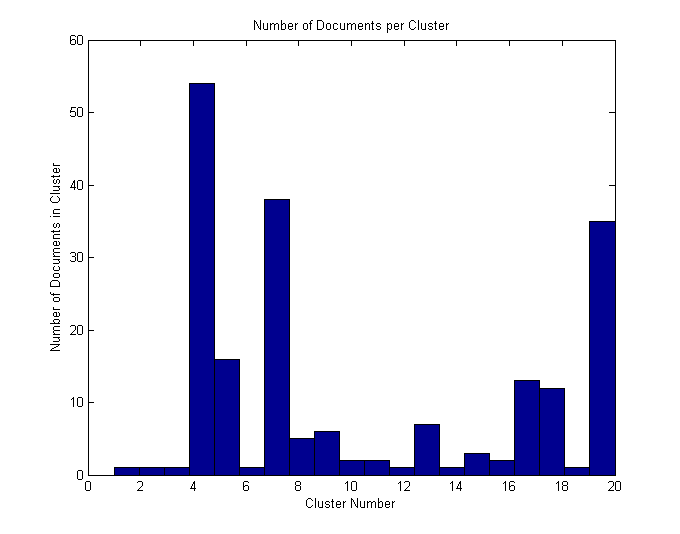
\includegraphics[width=6 in]{prob2PartC.png}
\caption{Histogram of Number of Articles Per Cluster}
\end{figure}

\newpage

Here are the first most likely words for each cluster:\\
Cluster 1: laredo border international mexico river american city green mayor rio \\
Cluster 2: feet square broadway seventh street side times avenue block million \\
Cluster 3: test end houston 000 0101 0102 100 1900 1900s 1968 \\
Cluster 4: millennium city night fireworks times 2000 midnight yeltsin russian friday \\
Cluster 5: y2k 2000 problems computer koskinen saturday computers system problem reported \\
Cluster 6: warrick heisman florida award guy national championship college field game \\
Cluster 7: american president national america war sports country 000 young white \\
Cluster 8: century book week school finds photographs 000 sales lives war \\
Cluster 9: game games goal million play going fortson team elias bruins \\
Cluster 10: home stay fathers children group child kids working called com\\ 
Cluster 11: archbishop bishop cardinal york church close leader late served american \\
Cluster 12: 2000 computer problem systems city failure officials 000 100 ahead \\
Cluster 13: bowden vick bowl coach florida game tech virginia football yards \\
Cluster 14: iqbal police 100 children apartment later month news story thursday\\ 
Cluster 15: season giants rusie game team 000 coach games players free \\
Cluster 16: buses authority diesel natural gas plan mta city york hybrid \\
Cluster 17: bradley candidates campaign mccain hampshire bush political president republican voters \\
Cluster 18: square times city economy york millennium 000 2000 mexico party \\
Cluster 19: lott players union executive player nfl think case challenge director \\
Cluster 20: team game season league players coach games play win teams \\
\\
Some of these seem to be interpretable sets. Cluster 17 seem to be politics related articles. Cluster 19 seem to be sports related articles. Other clusters though, such as cluster 3, do not seem to have a coherent theme. \\
\\
Here is the code to complete Part C. It relies on the code from the previous part: \\
\lstinputlisting[firstline=32, lastline=49]{prob2.m}

\newpage

\subsection*{Part d}

Here are the documents in the same cluster as document 1:\\
\lstinputlisting[firstline=1, lastline=131]{prob2PartD_1.txt}
These seem to all be related to sports. \\
\\
Here are the documents in the same cluster as 15:\\
\lstinputlisting[firstline=1, lastline=131]{prob2PartD_15.txt}
These seem to all be related to the Y2K phenomenon. \\
\\
Here is the cluster related to article 30:
\\
\lstinputlisting[firstline=1, lastline=131]{prob2PartD_1.txt}
These do not seem to be related

\end{document}
